\documentclass{beamer}

\usetheme{Singapore}
\usecolortheme{dove}
\usefonttheme{structurebold}
\usepackage{graphicx}
\usepackage{color}
\usepackage{xcolor}
\usepackage[british]{babel}
\usepackage[all]{xy}

\title[Plastic Soup recognition]{Plastic Soup recognition}
\subtitle[]{Project plan presentation}
\author[Y. Galama]{Student:\\Ysbrand Galama \\ 10262067 \\[2pc] Supervisor: Thomas Mensink\\}
\institute[UvA]
{
 
\includegraphics[width=0.7\textwidth]{images/uva-campus.pdf}
}
\date{24th April 2015}

\begin{document}

	\begin{frame}
	  \titlepage
	\end{frame}

\section{Introduction}
    \begin{frame}{Plastic Soup}
        \begin{itemize}
                \item Large amounts of plastic end up in the world ocean \cite{plastic}
                \item Automate the clean-up process
                \item Develop plastic soup recognition
        \end{itemize}
        \begin{columns}[c]
            \begin{column}{.5\textwidth}
            \end{column}
            \begin{column}{.5\textwidth}
                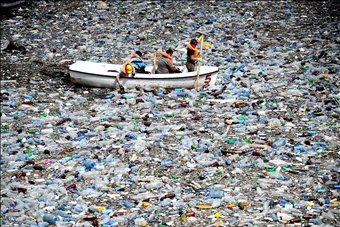
\includegraphics[width=\textwidth]{images/boat_in_plastic.jpg}\\{\small Figure 1: Boat in plastic soup}
            \end{column}
        \end{columns}
    \end{frame}
    
    \begin{frame}{Current state of the art image techniques}
        \begin{block}{Convolutional Neural Networks}
            \begin{itemize}
            \item Alexnet implementation to train large amounts of data \cite{alexnet}
            \item Current CNNs very high accuracy \cite{cnn}
            \end{itemize}
        \end{block}
        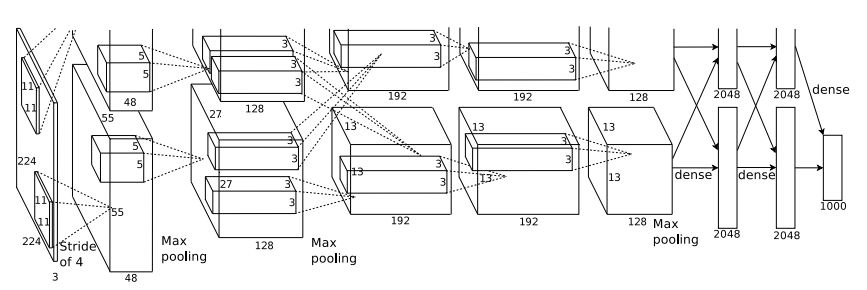
\includegraphics[width=\textwidth]{images/alexnet2012.png}
    \end{frame}
    \begin{frame}{Research question}
        \begin{block}{How does a pre-trained CNN perform when used for other classifications without being trained on a large amount of domain-specific data?}
            \begin{itemize}
            \item Assumes the high accuracy of CNNs
            \item Usage of pre-trained nets because of small dataset
            \end{itemize}
        \end{block}
    \end{frame}
\section{Method}
    \begin{frame}{Dataset}
        \begin{columns}[c]
            \begin{column}{.5\textwidth}
                \begin{itemize}
                \item 37165 images from short films
                \item annotated by hand
                \item 16553 images above and 20612 images below water
                \item 20635 show plastic only
                \item 6972 show animals only
                \item 8502 show both
                \end{itemize}
            \end{column}
            \begin{column}{.4\textwidth}
                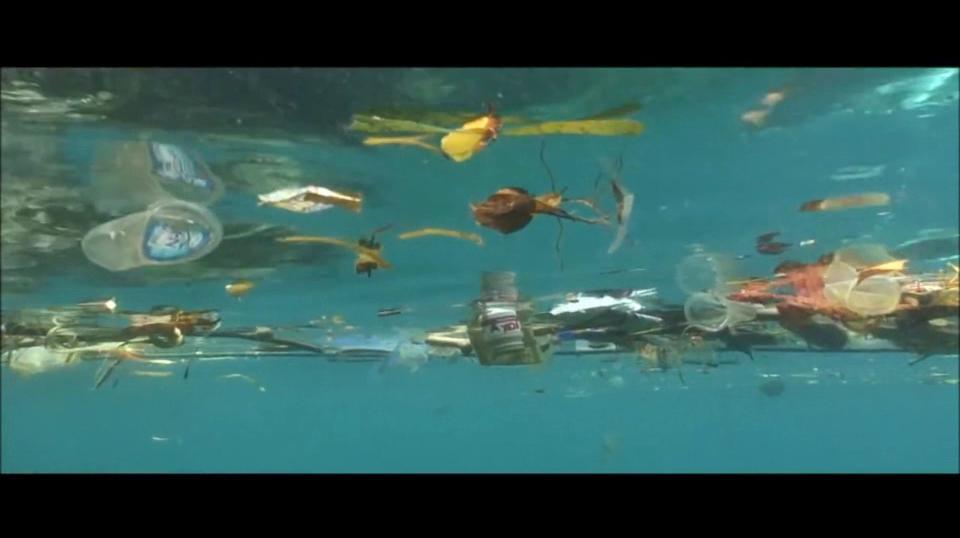
\includegraphics[width=\textwidth]{images/10947_01.jpg}\\
                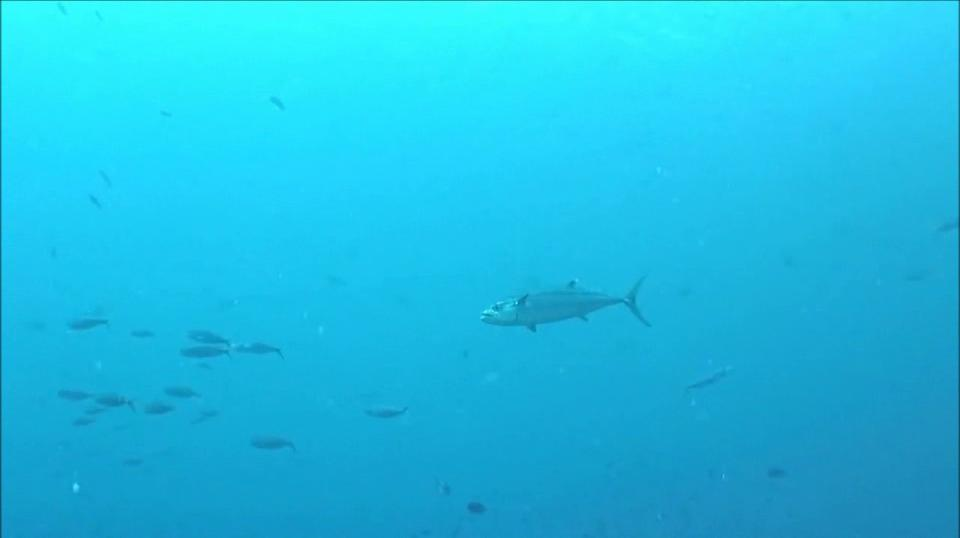
\includegraphics[width=\textwidth]{images/19358_10.jpg}\\
                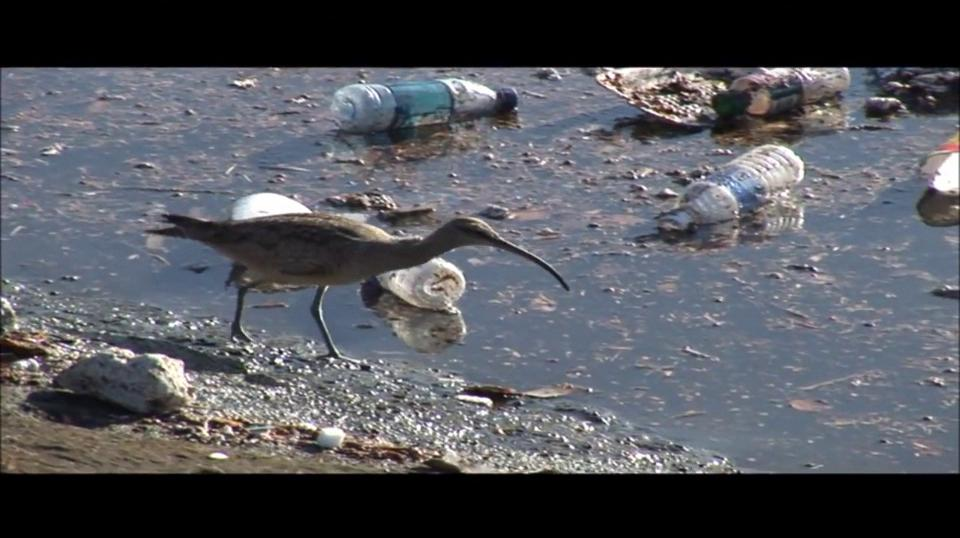
\includegraphics[width=\textwidth]{images/9077_11.jpg}\\
            \end{column}
        \end{columns}
    \end{frame}
    
    \begin{frame}{Method and evaluation}
        \begin{block}{Approach}
            \begin{itemize}
            \item Usage of a pre-trained Convolutional Neural Network
            \item Retrain the last layer for this specific domain
            \end{itemize}
        \end{block}
        \begin{block}{Evaluation}
            \begin{itemize}
            \item split dataset in train, validate and test
            \item score the results on the annotated data
            \end{itemize}
        \end{block}
    \end{frame}

\section{Plan}
    \begin{frame}{Plan}
        \xymatrix{
        {\begin{array}{l}
            \text{Collect and annotate data} \\
            \text{Install CNN framework}
        \end{array}} \ar[d] & \\
        {\begin{array}{c}
            \text{Classify last layer of CNN}\\
            \text{(2 weeks)}
        \end{array}} 
        \ar[d]_{baseline}^{satisfactory} \ar[dr]^{baseline}_{not\;satisfactory}
        & \\
        {\begin{array}{c}
            \text{Find plastic within image} \\
            \text{(4 weeks)}
        \end{array}}
        \ar[dr] & 
        {\begin{array}{c}
            \text{Use other texture-based} \\
            \text{imaging  techniques} \\
            \text{(4 weeks)}
        \end{array}}\ar[d] \\
        & 
        {\begin{array}{c}
            \text{write report} \\
            \text{(2 weeks)}
        \end{array}}
        }
    \end{frame}

    \begin{frame}[allowframebreaks]{References}
        \bibliographystyle{abbrv}
        \bibliography{Tex_sources/beamerbib}
    \end{frame}
\end{document}